\documentclass[presentation]{beamer}
\usepackage{presentation-slides}
\usepackage[english]{babel}
\usepackage[utf8]{inputenc}
\usepackage{beamersapere}
\usepackage[active]{srcltx}
\usepackage{alltt, fancyvrb, url, listings}
\usepackage{amsmath,amssymb,stmaryrd,mathtools,alltt,fancyvrb,url}
\usepackage{cleveref}
\usepackage{tikz}
\usepackage{array}
\usepackage{subcaption}


\usepackage{multimedia}
\usepackage[normalem]{ulem}

%\usepackage[style=verbose,autocite=footnote,maxnames=10,babel=hyphen,hyperref=true,abbreviate=false,backend=bibtex,mcite]{biblatex}
%\usepackage{calculus}

%%%% Title
\title[HPC from a self-org perspective]{HPC from a self-organisation perspective:\\ the case
of crowd steering at the urban scale}
%%%% Subtitle
%%%% Authors
\author[Pianini, Viroli, Zambonelli, Ferscha]
{Danilo Pianini$^1$, \textbf{Mirko Viroli$^1$}, Franco Zambonelli$^2$, Alois Ferscha$^3$}
%%%% Institution/Partner
\institute[] {
  $^1$\textsc{Alma Mater Studiorum}---Universit{\`a} di Bologna, Italy\\
  \texttt{\{danilo.pianini | mirko.viroli\}@unibo.it} \\
  ~\\
  $^2$Università degli Studi di Modena e Reggio Emilia, Italy\\
  \texttt{franco.zambonelli@unimore.it} \\
  ~\\
  $^3$Johannes Kepler University, Austria\\
  \texttt{ferscha@pervasive.jku.at}
}

%%%% Date
\date[July 22 2014]{Bologna, July 22 2014}


\begin{document}

%%% Syntax


\newcommand{\BNFcce}{{\bf ::=}}
\newcommand{\BNFmid}{\;\bigr\rvert\;}

\newcommand{\PROGRAM}{\texttt{P}}
\newcommand{\FUNCTION}{\texttt{F}}
\newcommand{\e}{\texttt{e}}
\newcommand{\fname}{\texttt{f}}
\newcommand{\xname}{\texttt{x}}
\newcommand{\yname}{\texttt{y}}
\newcommand{\oname}{\texttt{o}}
\newcommand{\pe}{\texttt{p}} % pure expression
\newcommand{\we}{\texttt{w}} % variable or (local) value




\newcommand{\asuper}{\texttt{s}}
\newcommand{\avalue}{\texttt{v}}
\newcommand{\bvalue}{\textit{b}}
\newcommand{\obvalue}{\option{\bvalue}}
\newcommand{\lvalue}{\texttt{l}}
\newcommand{\olvalue}{\option{\lvalue}}
\newcommand{\nvalue}{\texttt{n}}
\newcommand{\tvalue}{\texttt{t}}
\newcommand{\hvalue}{\texttt{h}}
\newcommand{\fvalue}{\phi}
\newcommand{\nolabel}{\_}
\newcommand{\fdom}[1]{\textit{dom}(#1)}
\newcommand{\oexec}{\epsilon}

\newcommand{\brvalue}{\textit{b}}
\newcommand{\obrvalue}{\option{\brvalue}}
\newcommand{\lrvalue}{\textit{l}}
\newcommand{\olrvalue}{\option{\lrvalue}}

\newcommand{\tvalueExt}[1]{(\lvalue_1,\ldots,\lvalue_{#1})}
\newcommand{\fvalueExt}[2]{\{#1\mapsto #2\}}
\newcommand{\fvalueOne}[2]{\{#1\mapsto #2\}}
\newcommand{\fvalueWrap}[1]{\{#1\}}
\newcommand{\fvaluewrapped}[2]{#1\mapsto #2}
\newcommand{\fvalues}[2]{#1\mapsto #2}
%\newcommand{\memslot}[2]{\{#1:=#2\}}
\newcommand{\memslot}[2]{#1:=#2}
\newcommand{\treeslot}[2]{#1\mapsto #2}
\newcommand{\emptyL}{\bullet}

\newcommand{\avalueSet}{\mathcal{V}}
\newcommand{\lvalueSet}{\mathcal{L}}
\newcommand{\nvalueSet}{\mathcal{N}}
\newcommand{\tvalueSet}{\mathcal{T}}
\newcommand{\hvalueSet}{\mathcal{H}}
\newcommand{\fvalueSet}{\Phi}
% Keywords
\newcommand{\defK}{\texttt{def}}
\newcommand{\nbrK}{\texttt{nbr}}
\newcommand{\repK}{\texttt{rep}}
\newcommand{\ifK}{\texttt{if}}

\newcommand{\tname}{\texttt{t}}

\newcommand{\ltrue}{\textit{t}}
\newcommand{\lfalse}{\textit{f}}


%%% Runtime Syntax

\newcommand{\wildcard}{{\cdots}} %%% non intresting syntact element
%\newcommand{\option}[1]{{{#1}_\mathit{opt}}} %%% optional syntact element
\newcommand{\option}[1]{\mathring{#1}} %%% optional
\newcommand{\evaluatedPlace}{{\place_\mathit{top}}} %%% optional syntact element
%%%\newcommand{\re}{\textit{r}} %%% runtime expression
\newcommand{\re}{\textit{a}} %%% runtime expression
\newcommand{\rv}{\textit{v}} %%% runtime value
\newcommand{\lre}{\textit{e}} %%% labeled runtime expression
\newcommand{\olre}{\option{\lre}} %%% optional labeled runtime expression
%%%\newcommand{\orv}{\textit{w}}  %%% optional runtime value
\newcommand{\orv}{\option{\rv}}  %%% optional runtime value
\newcommand{\ob}{\textit{b}}  %%% optional body
\newcommand{\Env}{\Gamma}
\newcommand{\emptyEnv}{\bullet}
\newcommand{\Trees}{\Theta}
\newcommand{\emptyTrees}{\bullet}
\newcommand{\labelled}[2]{#1\!\!\cdot\!\!{#2}}
\newcommand{\labelledsmall}[2]{#1\cdot{#2}}
\newcommand{\labelledC}[2]{#1^{#2}}
\newcommand{\labelledCsmall}[2]{#1^{#2}}

\newcommand{\he}{h} %%%  local value or runtime expression
\newcommand{\ohe}{\option{\he}} %%% optional local value or runtime expression
\newcommand{\ue}{\textit{u}} %%% unevaluated runtime expression
\newcommand{\uhe}{\option{\ue}} %%% optional unevaluated runtime expression

\newcommand{\unfoldK}{\texttt{unfold}}

\newcommand{\newopsem}[5]{#1;#2;#3\vdash #4\rightarrow #5}
\newcommand{\opsem}[4]{#1;#2\vdash #3\rightarrow #4}
\newcommand{\opsemmany}[4]{#1;#2\vdash #3\rightarrow^* #4}
\newcommand{\opsemNF}[3]{#1;#2\vdash #3\not\rightarrow}

\newcommand{\self}{\texttt{self}}

%%% Alignment contexts

\newcommand{\actx}{\mathbb{A}}
\newcommand{\matches}{::}

%%% Contexts

\newcommand{\ctxapp}[2]{#1[#2]}
\newcommand{\ctxappfull}[3]{\ctxapp{#1}{#2}\langle #3\rangle}
\newcommand{\ctx}{\mathbb{C}}
\newcommand{\ctxr}{\mathbb{R}}
\newcommand{\ctxf}{\mathbb{N}}
\newcommand{\ctxc}{\mathbb{C}}
\newcommand{\ctxrt}{\mathbb{RT}}
\newcommand{\ctxt}{\mathbb{T}}
\newcommand{\ctxre}{\mathbb{RE}}
\newcommand{\ctxe}{\mathbb{E}}
\newcommand{\hole}{[]}
\newcommand{\place}{\langle\rangle}
\newcommand{\placefilled}[1]{\langle #1\rangle}
\newcommand{\inversectx}[2]{\spi{#1}(#2)}
\newcommand{\spi}[1]{\pi_{#1}}
\newcommand{\erase}[1]{|#1|}

\newcommand{\transition}[3]{
  \begin{array}{l@{\;}c}
    \stackrel{~}{{\tiny \textrm{[#1]}}} & #2 \\ \hline
    \multicolumn{2}{c}{#3}
  \end{array}
}
\newcommand{\transitiontwoprec}[4]{
  \begin{array}{l@{\qquad}c}
    & #2\\
    {\tiny \textrm{[#1]}} & #3 \\ \hline
    \multicolumn{2}{c}{#4}
  \end{array}
}
\newcommand{\nulltransition}[2]{
  \transition{#1}{}{#2}
}

\newcommand{\smallerskiptransition}{\\[-4pt]}
\newcommand{\smallskiptransition}{\\[0pt]}
\newcommand{\skipreduction}{\\}
\newcommand{\skiptransition}{\\[10pt]}
\newcommand{\bigskiptransition}{\\[15pt]}

\newcommand{\sta}{\textit{s}}
\newcommand{\stat}[4]{\langle#1,#2,#3,#4\rangle}
\newcommand{\topStat}[3]{\langle#1,#2,#3\rangle}
\newcommand{\tstat}[5]{#1\!::\!\langle #2,#3,#4,#5\rangle}
\newcommand{\msg}[2]{\{#1\rhd #2\}}
\newcommand{\fullmsg}[3]{#1:#2\rhd #3}
\newcommand{\sys}{\textit{N}}
\newcommand{\opar}{\;||\;}
\newcommand{\opard}{\oplus}
\newcommand{\lab}{\lambda}
\newcommand{\labtau}[1]{#1:\tau}
\newcommand{\labstart}[2]{#1\uparrow #2}
\newcommand{\labstop}[3]{#1\downarrow(#3) #2}
\newcommand{\upd}[2]{#1[#2]}
\newcommand{\replace}[2]{#2\rhd #1}
\newcommand{\proj}[2]{{#1}|_{#2}}
\newcommand{\topo}{\varSigma}
\newcommand{\envmap}[2]{\{#1\mapsto #2\}}

\newcommand{\fromMsg}[2]{\mathit{from}(#1,#2)}
\newcommand{\toMsg}[2]{\mathit{to}(#1,#2)}

\newcommand{\initNAME}{\textit{init}}
\newcommand{\init}[1]{\initNAME(#1)}
\newcommand{\ruleNameSize}[1]{{\scriptsize #1}}


% Code highlighting
\newcommand{\il}[1]{{\it \textcolor{gray}{;; #1}}} % inline comment
\newcommand{\km}[1]{{\bf \textcolor{red}{#1}}} % key mechanism primitives
\newcommand{\fn}[1]{\textcolor{blue}{#1}} % function calls
\newcommand{\pr}[1]{\textcolor{magenta}{#1}} % primitives


\frame[label=coverpage]{\titlepage}
\newcommand{\jkuthanks}{\vspace{-20pt}{\Tiny (Pict. by A. Ferscha, JKU)}}
\newcommand{\comment}[1]{}

\begin{frame}\frametitle{High performance computing}
  \begin{block}{A possible definition}
    Aggregation of computational capabilities in such a way that intense computations can be executed in a much shorter time than it would require on a classic end-user machine.
  \end{block}
  \begin{block}{General perception}
    Building size, centralised and massively parallel machines, that compute based on data users send them.
  \end{block}
    \begin{figure}
      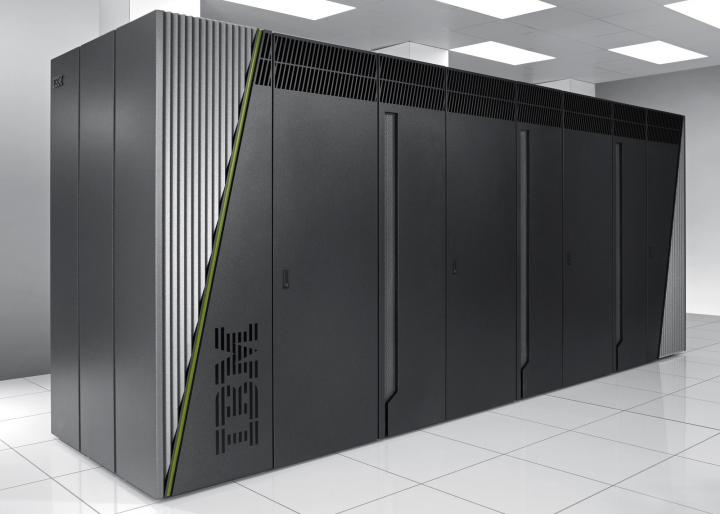
\includegraphics[width=4.5cm]{img/fermi}\\
      \Tiny{CINECA's ``Fermi'' super computer}
    \end{figure}
\end{frame}

\begin{frame}\frametitle{HPC from a different perspective}
  \begin{block}{A different point of view}
    \begin{itemize}
     \item Massively parallel
     \item \sout{Centralised} --- Distributed
     \item \sout{Building-size} --- City-size
     \item \sout{Receives data from a source} --- Perceives data from the surroundings
    \end{itemize}
  \end{block}
  \begin{block}{Our position}
    We argue that, if equipped with proper communication technology, our smartphones, tablets, wearable devices and all the objects with computational abilities spread in a urban environment (public screens, sensors, cameras) constitute a ``high performance computing system at the urban scale''.
  \end{block}
\end{frame}

\begin{frame}\frametitle{What kind of computation?}
  \begin{block}{Locality}
    Some computations require local, contextual information. Some simple examples:
    \begin{itemize}
     \item Determining how crowded are the areas near me, in order to decide which way is faster
     \item Knowing whether and where someone is in a crowded room or not
     \item During an emergency, promptly react to contingencies not considered in the evacuation plan, e.g. because of a broken stair
    \end{itemize}
  \end{block}
  \begin{block}{Our position}
    There is a wide space for applications in which contextual information is only locally relevant: in those cases the global behaviour can be achieved by spreading the computation among the nodes participating the system in that specific spatio-temporal frame, with no need of a centralised computing system.
  \end{block}
\end{frame}

\begin{frame}\frametitle{An urban event scenario}
  \begin{block}{Proof of concept}
    We want to exemplify the concept by an example.
  \end{block}
  \begin{block}{Crowd sensitive navigation}
    Steer people towards their goal circumventing over-crowded areas, in order to reduce trip time and improve overall security
    \begin{itemize}
     \item Different from per-user navigation: we need the current position of people along the possible paths, and we want to be reactive to changes.
    \end{itemize}
  \end{block}
\end{frame}

\begin{frame}\frametitle{Devices and physical configuration}
  \begin{block}{Our assumptions}
    \begin{itemize}
     \item Each user is equipped with a smart device
     \item Each device is aware of its own position
     \item Some object deployed in the city, e.g. public screens and semaphores, are equipped with ``static'' devices that participate the computation
     \item Each mobile device can communicate with the closest static device, if there is any within its communication certain range
     \item Each static device can sense how many mobile devices are connected
     \item Each static device can communicate with other static devices within a certain communication range
    \end{itemize}
  \end{block}
\end{frame}

\begin{frame}\frametitle{Distributed crowd steering I}
  \begin{block}{Spatial gradient}
    \begin{itemize}
     \item Distributed data structure
     \item It assigns to each node a space-time dependent value $\varGamma$
     \item It originates in one or more devices called sources
     \item In every source device, $\varGamma=0$.
     \item In every other device, $\varGamma=[\min(f(n)) | n \in N]$: namely, the value of the device is the minimum of a function which operates on the neighbours.
     \item Along with the local value, a gradient can carry more information, e.g. some strings, the position of $n$, or numeric values
    \end{itemize}
  \end{block}
  \begin{block}{Example}
    If $f(n) = \varGamma_{n} +d(n)$ where $d(n)$ measures the actual distance from the device towards $n$, then the value of the gradient will approximate the distance from the nearest source.
  \end{block}
\end{frame}

\begin{frame}\frametitle{Distributed crowd steering II}
  \begin{block}{Basic steering}
    \begin{itemize}
     \item The device wanting to be steered publishes a gradient including the information about the wanted destination
     \item One or more static devices located near a potential point of interest (POI) receive such gradient, and react becoming sources of a gradient which measures the distances between nodes
     \item This response gradient diffuses on static nodes until it reaches the source, carrying within itself information about the chain of static devices forming the shortest path
     \item The requester will receive a gradient pointing towards the nearest POI, and can navigate step-by-step by reaching in order all the nodes of the path
    \end{itemize}
  \end{block}
\end{frame}

\begin{frame}\frametitle{Distributed crowd steering III}
  \begin{block}{Crowd sensitive steering}
    \begin{itemize}
     \item Let's call $C$ the perceived number of mobile devices surrounding a static node
     \item We can alter the spatial shape of the gradient by e.g. adopting $f(n) = \varGamma_{n} +d(n) + K\dot C$ where $K$ is a system parameter
    \end{itemize}
  \end{block}
  What happens? Basically, areas densely populated with mobile devices will appear as more distant, and consequently the requester will be steered towards alternative routes
\end{frame}

\begin{frame}\frametitle{Real life scenario}
  \begin{block}{Vienna City Marathon 2013}
    \begin{itemize}
     \item Mass urban sports event
     \item Involves every year about 40.000 actives and 300.000 spectators
     \item During such event, a smartphone application based on SAPERE \cite{sapere-procedia7} concepts was deployed, and gathered 1503 high quality GPS traces \cite{socinfo2013}
     \item We relied on such data set to build simulations
    \end{itemize}
  \end{block}
\end{frame}

\begin{frame}\frametitle{Simulation setup}
  \begin{block}{The tool: Alchemist}
    \begin{itemize}
     \item A simulator whose engine was inspired by exact stochastic simulators for chemistry, but whose model is designed to support the simulation of distributed computational system \cite{alchemist-jos2013}
     \item The simulator supports loading maps and data from OpenStreetMap \cite{osm}
     \item Ships with a module based on GraphHopper\footnote{\url{http://graphhopper.com/}} which provides the simulator the ability to compute routes between two points of the map
     \item Allows for loading GPS traces
    \end{itemize}
  \end{block}
\end{frame}

\begin{frame}\frametitle{Simulation snapshot}
  \begin{figure}
    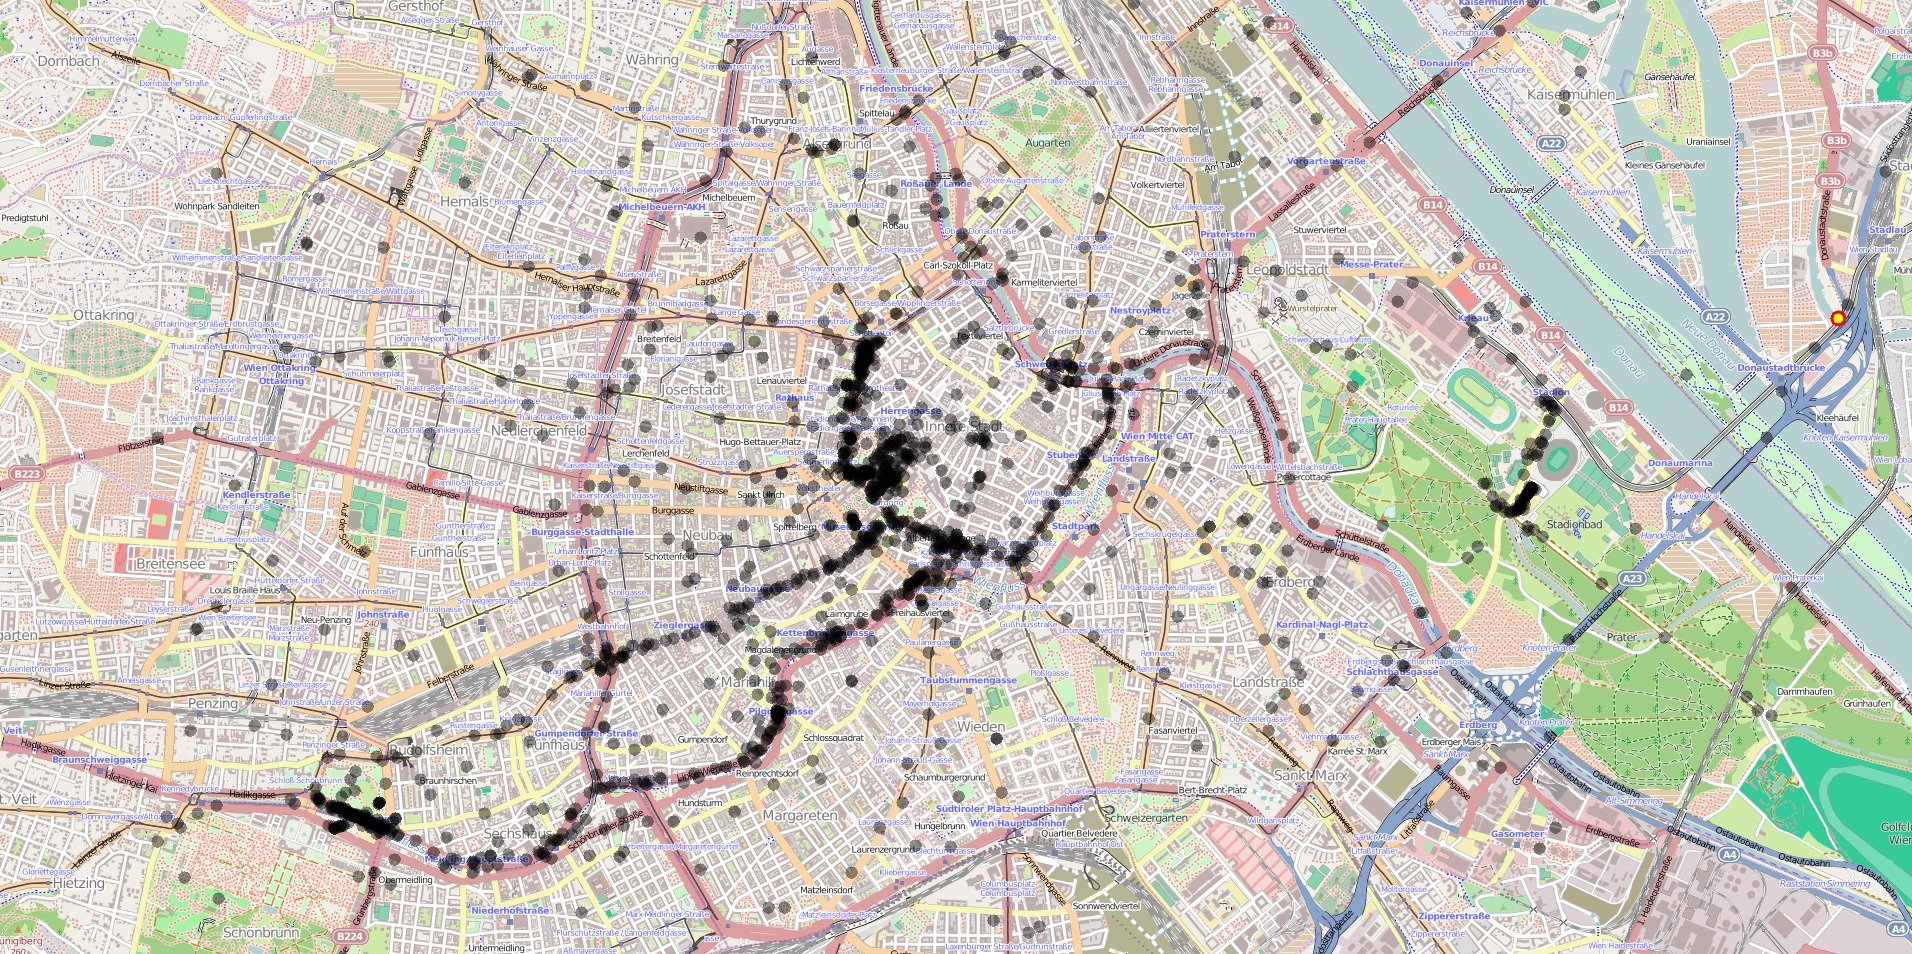
\includegraphics[width=0.99\textwidth]{img/vienna}
    \caption{A snapshot of the whole city of Vienna as simulated in Alchemist. This snapshot is taken while simulating the city at 10am, each black point corresponds to a GPS trace. The more an area is crowded, the blacker it appears in the image.}
    \label{img:vienna}
  \end{figure}
\end{frame}

\begin{frame}\frametitle{Crowd sensitive steering benefits: example}
  \begin{figure}
  \begin{subfigure}[b]{0.325\textwidth}
   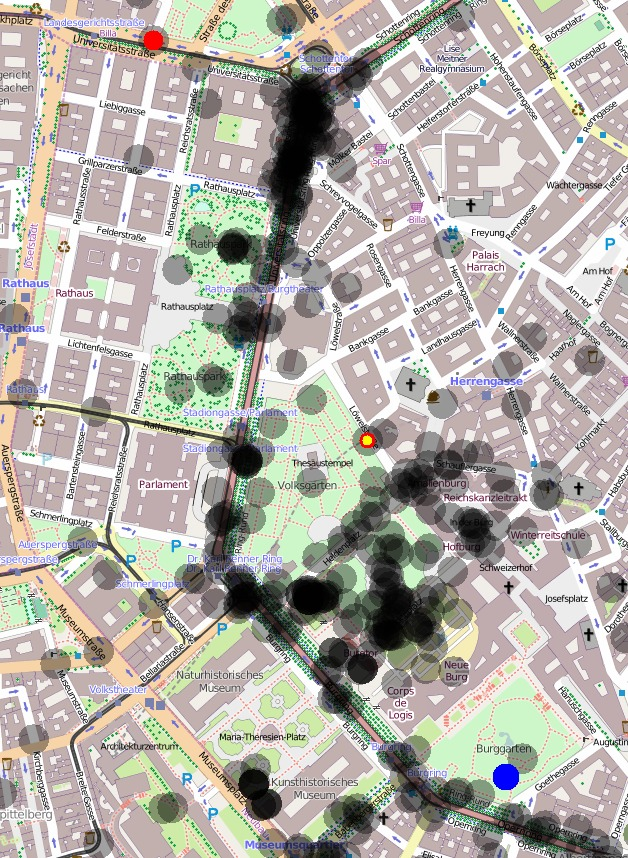
\includegraphics[width=\textwidth]{img/crowd}
   \caption{Crowding level}
   \label{img:crowd}
  \end{subfigure}
  \begin{subfigure}[b]{0.325\textwidth}
   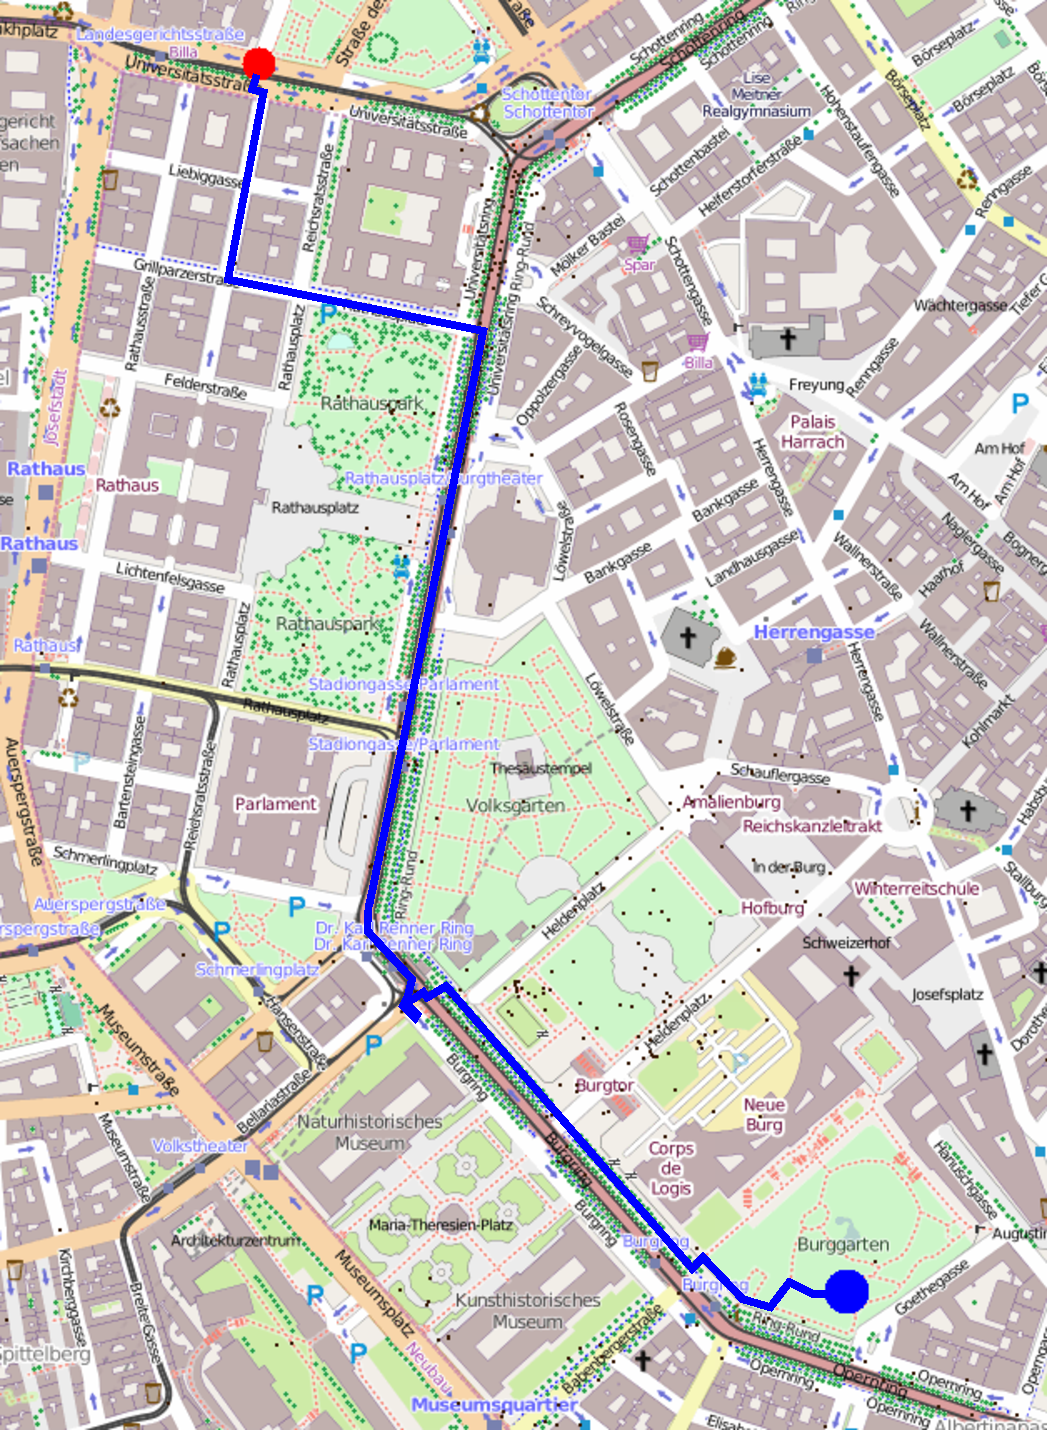
\includegraphics[width=\textwidth]{img/vcm_nocd2}
   \caption{Classic}
   \label{img:nocrowd}
  \end{subfigure}
  \begin{subfigure}[b]{0.325\textwidth}
   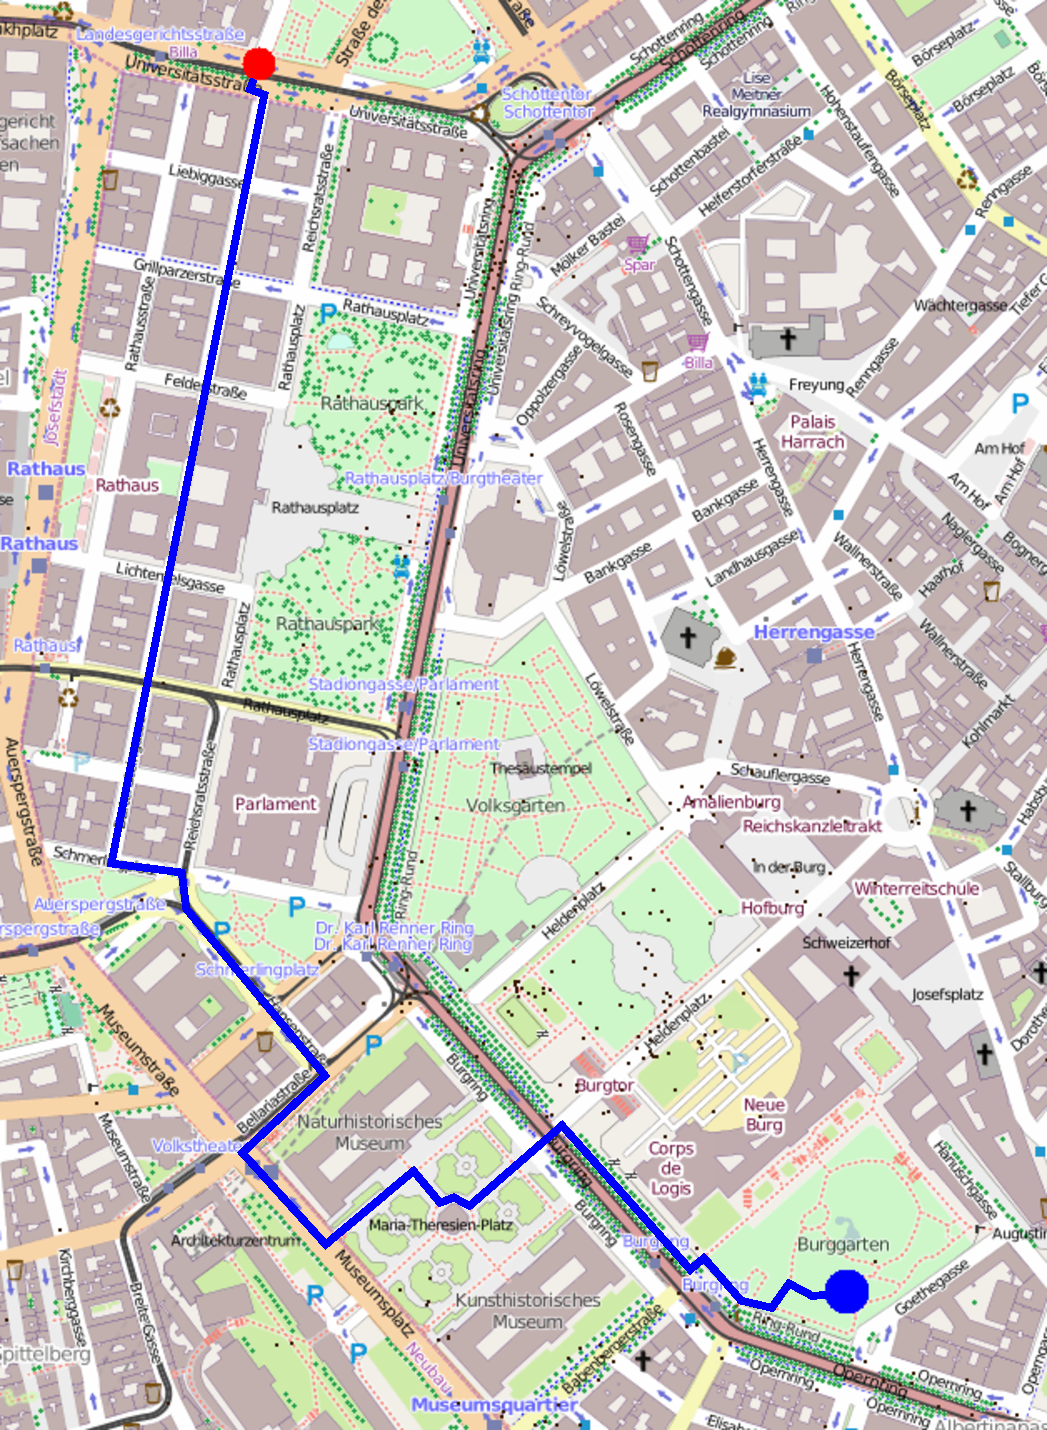
\includegraphics[width=\textwidth]{img/vcm_cd}
   \caption{Crowd-sensitive}
   \label{img:crowdsteering}
  \end{subfigure}
  \end{figure}
\end{frame}

\begin{frame}\frametitle{Crowd sensitive steering benefits: data}
  \begin{figure}
  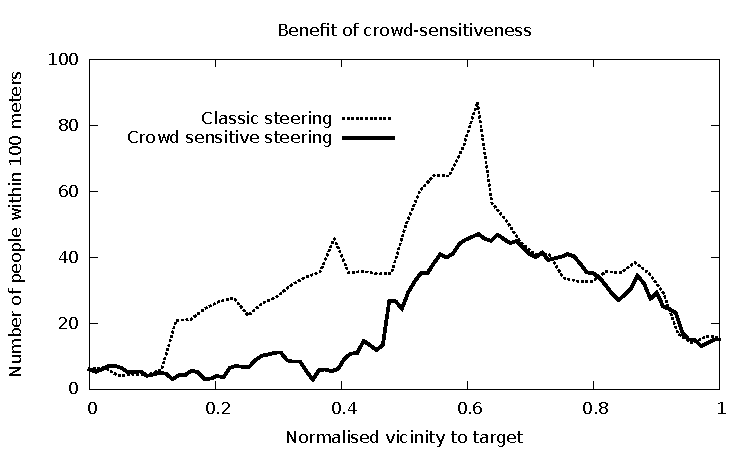
\includegraphics[width=0.99\textwidth]{img/chart}
  \end{figure}
  \Tiny{Number of users surrounding the user (within 100 meters from her).
  %
  With ``normalised distance'', we mean that we divided the distance the user still has to walk to reach the target by the total length of the suggested path.}
\end{frame}

\bibliographystyle{apalike}
\setbeamertemplate{bibliography item}[text]
{\tiny \begin{frame}{References} 
\bibliography{bibliography}
\end{frame}}

\end{document}
